% ----------- Cover Master Thesis Faculty of Sciences ---------------
% This document should be compiled with pdflatex.  If you want to use
% latex to compile to dvi/ps, you have to convert the images to (e)ps
%                           -- December 2012
% -------------------------------------------------------------------
\RequirePackage{fix-cm}
\documentclass[12pt,a4paper,oneside]{book}

% ------------------------- Load packages ---------------------------
% You can eventually add these while you load other packages
% in case you want to integrate the titlepage with the rest of your thesis
% -------------------------------------------------------------------
\usepackage{graphicx,xcolor,textpos}
\usepackage{helvet}
\usepackage{hyperref}
\usepackage{makeidx}
%\usepackage{subfigure} % DEPRECATED
\usepackage{caption}
\usepackage{subcaption}
\usepackage[]{algorithm2e}
\usepackage{longtable}

% ------------------------ Page settings -----------------------------
% If you change these, the cover layout will also change.  In that
% case you have to adjust the latter manually.
% --------------------------------------------------------------------

\topmargin -10mm
\textwidth 160truemm
\textheight 240truemm
\oddsidemargin 0mm
\evensidemargin 0mm

% ---------------------- textpos settings ----------------------------
% Some additional settings for the cover
% --------------------------------------------------------------------

\definecolor{green}{RGB}{172,196,0}
\definecolor{bluetitle}{RGB}{29,141,176}
\definecolor{blueaff}{RGB}{0,0,128}
\definecolor{blueline}{RGB}{82,189,236}
\setlength{\TPHorizModule}{1mm}
\setlength{\TPVertModule}{1mm}

% ---------------------------- index ---------------------------------
%
% --------------------------------------------------------------------
\makeindex

\begin{document}

% ----------------------- Cover --------------------------------------
% Please fill in:
% - The title and subtitle (if applicable)
%         to include a formula in the title or subtitle
%         use  \form{$...$}
% - Your name
% - Your (co)supervisor, mentor (if applicable)
% - Your master
% - The academic year
% --------------------------------------------------------------------
\thispagestyle{empty}
\newcommand{\form}[1]{\scalebox{1.087}{\boldmath{#1}}}
\sffamily
%
\begin{textblock}{191}(-24,-11)
	\colorbox{green}{\hspace{139mm}\ \parbox[c][18truemm]{52mm}{\textcolor{white}{FACULTY OF SCIENCE}}}
\end{textblock}
%
\begin{textblock}{70}(-18,-19)
	\textblockcolour{}
	\includegraphics*[height=19.8truemm]{LogoKULeuven}
\end{textblock}
%
\begin{textblock}{160}(-6,63)
	\textblockcolour{}
	\vspace{-\parskip}
	\flushleft
	\fontsize{40}{42}\selectfont \textcolor{bluetitle}{Visualization of music suggestions}\\[1.5mm]
	\fontsize{20}{22}\selectfont {A visual explanation system for collaborative filtering}
\end{textblock}
%
%\begin{textblock}{82}(50,103)
%\textblockcolour{}
%\vspace{-\parskip}
%\flushleft
%\fbox{\parbox{79mm}{The background can be left blank or you can insert an image (maximum height 10 cm, width variable, mind author's rights). NO logos (you can use the logos inside the manuscript, but not on front or back cover). \textit{Delete this textbox.}}}
%\end{textblock}
%
\begin{textblock}{160}(8,153)
\textblockcolour{}
\vspace{-\parskip}
\flushright
\fontsize{14}{16}\selectfont \textbf{Joris SCHELFAUT}
\end{textblock}
%
\begin{textblock}{70}(-6,191)
\textblockcolour{}
\vspace{-\parskip}
\flushleft
Supervisor: Prof. E. Duval\\[-2pt]
\textcolor{blueaff}{Affiliation \textsl{(optional)}}\\[5pt]
Co-supervisor: \textsl{(J. Klerkx)}\\[-2pt]
\textcolor{blueaff}{Affiliation \textsl{(optional)}}\\[5pt]
Mentor: \textsl{(J. Klerkx)}\\[-2pt]
\textcolor{blueaff}{Affiliation \textsl{(optional)}}\\
\end{textblock}
%
\begin{textblock}{160}(8,191)
\textblockcolour{}
\vspace{-\parskip}
\flushright
Thesis presented in\\[4.5pt]
fulfillment of the requirements\\[4.5pt]
for the degree of Master of Science\\[4.5pt]
in Applied Computer Science\\
\end{textblock}
%
\begin{textblock}{160}(8,232)
\textblockcolour{}
\vspace{-\parskip}
\flushright
Academic year 2012-2013
\end{textblock}
%
\begin{textblock}{191}(-24,248)
{\color{blueline}\rule{550pt}{5.5pt}}
\end{textblock}
%
\vfill
\newpage

% In case you want to integrate the TeX-file for the titlepage
% with the rest of your thesis, you cab continue below
% ------------------------- First pages ---------------------------
% For table of contents, acknowlegments, ...
% -----------------------------------------------------------------
\rmfamily
\setcounter{page}{0}
\pagenumbering{roman}

\newpage
\tableofcontents

\newpage
% -------------------------- Proper text --------------------------
% Introduction, chapters, ...
% -----------------------------------------------------------------
\setcounter{page}{0}
\pagenumbering{arabic}

%% TEX FILES (Chapters)
\chapter{Introduction}\label{chapter:introduction}

\section{Music suggestions and explanation systems}\label{chapter:introduction:section:context}

Imagine you have a music library with a number of tracks in it. No doubt you will like certain tracks more than others. At a certain point you will want to expand your library. It is only natural that you will want to add music that is similar to the music you already like, but where should you begin to look for this kind of music? Over the last decade, systems have been developed to compute what tracks, or in the more general case, items or information, would be of interest to you based on your listening history and/or track ratings. These kind of systems are called recommender systems.

In their essence, recommender systems can be seen as filters applied on a large data sets. Ever since computer engineers started to develop this kind of systems, a wide range of algorithms have been designed and implemented to compute item recommendations\cite{burke:2002, melville:2002:CCF:777092.777124, pazzani:2007:CRS:1768197.1768209, rajaraman:2012}; each of them with their own advantages and disadvantages.

Let us assume you have plugged some recommender system into your music library and you have received a list of music suggestions. Which of these recommendations should you choose? Of course you could go through them all one by one, but that might take up quite some time. What it comes down to is that you don't know how the recommender system computed these recommendations, and as a result, you have a hard time making an educated decision where to start.

To solve this problem, you will need some kind of explanation system that provides a reasoning to arrive at the results. An ambitious approach would be to explain each step of the recommendation algorithm, but this not always possible or desired. Indicating which of your tracks are closely related to the given recommendations, the system's confidence in the accuracy of the suggestions, et cetera, also help giving some additional context in explaining why a particular recommendation would be interesting\cite{herlocker:2000}. Over the course of the last decade a wide range of explanation systems have been implemented. Many of these also use visualizations to explore user and/or item relationships\cite{bostandjiev:2012, crnovrsanin:2011:VRN:2421953.2422013, faridani:2010:opinionspace, gou:2011:SIF:2016656.2016671, gretarsson:2010, odonovan:2008}.

Let's say that you have installed the the recommender system with an integrated explanation system. The explanation system visualizes how the items in your library are related to the recommendations, and provides additional statistics. Now, finding new, interesting music will hopefully become easier than ever before.

\section{Thesis objective}\label{chapter:introduction:section:objective}

The goal of this thesis is to design, implement and evaluate visualization and interaction techniques that will allow the user to gain insight into the recommendation process as well as actively steer the process. The elaboration of this thesis consists out of a literature study on the topic of visualization of music suggestions, and secondly a similar application that is designed and implemented\cite{kuleuven:2008:t313}.

In the design of the application findings of the literature study and comparative study of visual explanation systems are taken into account. From this initial design a hypothesis and expected result are derived. This hypothesis is tested through user tests. If possible, the application is improved. This process can be repeated, incrementally improving the application.

The scenario in section \ref{chapter:introduction:section:context} sketches the context in which this application can be used.


\section{A multi-focal perspective}\label{chapter:introduction:section:perspective}

Although the focus of this thesis lies on the creation of a visual explanation system for music recommendation, this thesis covers aspects of several research domains. Therefore, this text can be viewed from a multi-focal perspective. The various facets that can be distinguished are as follows: item recommendation, which is in turn a subfield of data mining, insight gaining and sensemaking, and information visualization and visual data mining. Also the graph drawing problem is an important topic in this paper. And last but not least, human-computer interaction can be seen as the overarching concept.

To make the forementioned topics more concrete in the context of this thesis, the following subsections try to explain how each of these topics is relevant, as well as explain how they are interrelated.


\subsection{Item recommendation}\label{chapter:introduction:section:perspective:subsection:recommendation}

Recommender systems form one of the major topics of this thesis. In particular this thesis tries to address the black box problem. In a paper by Herlocker et al. \cite{herlocker:2000}, recommender systems are compared to a black box. This black box generates item recommendations seemingly at random, leaving the user guessing as to how recommendations were computed. Herlocker et al. propose to create an explanation system, i.e., the white box, to overcome this black box problem.

Although there are many variations of recommendation algorithms, the focus of this thesis is on collaborative filtering-based (CF) item recommendation. This algorithm is studied in the context of music recommendation. The CF algorithm tries to establish similarities between user profiles, in this case music libraries with additional listening history and/or item ratings. Items in the difference between items sets of similar profiles are then candidate recommendations\cite{rajaraman:2012}.


\subsection{Insight gaining and sensemaking}\label{chapter:introduction:section:perspective:subsection:sensemaking}

Another aspect of this thesis is related to insight gaining. In order to develop an explanation system, it is interesting to explore how a user arrives at insight. We will try to define the insight gaining process and the related concept of sensemaking. Sensemaking is not uniquely defined as its meaning may slightly vary depending on the context\cite{yi:2008}. In short, sensemaking can be explained as the effort by an individual to understand the underlying information structures with the objective to answer task-specific questions\cite{russell:1993:CSS:169059.169209, yi:2008}.


\subsection{Information visualization and visual data mining}\label{chapter:introduction:section:perspective:subsection:infovis}

As the explanation system will be using visual elements, concepts from the field of information visualization will be used. We will look at general characteristics of information visualization and interactive visualization. Also, various visualization techniques, and clutter reduction techniques are discussed.


\subsection{Graph drawing}\label{chapter:introduction:section:perspective:subsection:graph}

To determine whether or not graphs are applicable to visualize a concept, Herman et al. \cite{herman:2000} pose the following question: "is there an inherent relation among the data elements to be visualized?" As the structure behind collaborative filtering can be interpreted as a network of users and items, the answer to this question is yes. As a result, it should come as no surprise that graphs are a popular way to visualize collaborative filtering-based recommendation\cite{bostandjiev:2012, gretarsson:2010}, and the application developed for this thesis will also contain a graph-based visualization.

Herman et al. \cite{herman:2000} define the graph drawing problem as follows: "given a set of nodes with a set of edges (relations), calculate the position of the nodes and the curve to be drawn for each edge". This thesis can then be seen as an effort to solve the graph drawing problem in a particular context, i.e., specific constraints in terms of screen size, data dimensionality, data quantity, et cetera.


\subsection{Human-computer interaction and usability}\label{chapter:introduction:section:perspective:subsection:hci}

In its most basic form, this is a thesis about humans and computers. The human uses a computer to find new item recommendations. The computer provides these recommendations. The human wants to understand the recommendation process. The computer explains how it computed the item suggestions. The user interacts with the system to further his/her understanding of the subject.

In this thesis we will try to understand the user, the system or computer, and the interface that allows interactions between them. Human interaction (CHI) is defined as "is the study of how people design, implement, and use interactive computer systems and how computers affect individuals, organizations and society."\cite{tripathi:2011}.

To improve the interaction between humans and computers, we will aim to develop an interface with high usability. The evaluation methods in this thesis draw from the evaluation techniques from the field of human-computer interaction. Paper prototyping, think aloud protocol, subjective evaluation methods among others, are examples of these techniques\cite{nielsen:1993:UE:529793}. In this sense, this thesis can be seen as a case study of designing, implementing and incrementally improving an application using CHI techniques.


\section{The visual explanation system}\label{chapter:introduction:section:application}

The application created for this thesis is a page action Chrome Extension that injects \emph{HTML} and \emph{JavaScript} into the recommendations page of \emph{Last.fm} at \url{http://last.fm/home/recs}. The application makes use of several \emph{JavaScript} libraries, such as D3\footnote{A library using SVG, HTML and JavaScript\cite{bostock:2012:d3js}; available at: \url{http://d3js.org/}} and jQuery\footnote{Available at: \url{http://jquery.com/}}, as well as a specific JavaScript library by Felix Bruns\footnote{Available at: \url{https://github.com/fxb/javascript-last.fm-api}} to facilitate the usage of the Last.fm API\footnote{Available at: \url{http://www.last.fm/api}}.

The application can be found in the Google Chrome web store\footnote{The SoundSuggest application can be found at: \url{https://chrome.google.com/webstore/detail/soundsuggest/jimmblcjmmjjfaklclmohcnabndlidmb}}.


\section{Next chapters}\label{chapter:introduction:section:chapters}

The rest of this thesis text is organized as follows. First we will present a literature study on the topics discussed in section \ref{chapter:introduction:section:perspective} of this introduction. The next chapter is a comparative study of recommender systems with visual explanation systems. After this we will try to design a white box for CF-based recommendation by applying some of the conclusions and techniques discussed in the literature study. This concludes the theoretical part of the thesis.

In the next part of the thesis we will look at the evaluation of the application's design through user tests, as well as the software design and implementation of the application. In these chapters we will try to identify liabilities in the design, highlight implementation details, and discuss evaluation methods.

The thesis text ends with an analysis of the application's evaluation results, further conclusions, and a reflection on future work and opportunities.

\chapter{Literature study}\label{chapter:literature_study}

The term 'human-computer interaction' describes a phenomenon where two actors, the human or \emph{user} and the computer or \emph{system}, share a communication channel. The communication channel is a representation of data of the system towards the user. It is clear that both actors will impose certain restrictions on this visual communication channel\cite{shirley:2009, ware:2004}. In this chapter we will try to establish who these actors are, what this communication channel looks like, and what kind of restrictions are imposed upon the visual communication channel. 



% --------------------------- The User ----------------------------
% 
% -----------------------------------------------------------------
\section{The user}\label{chapter:literature_study:section:user}

Who is the first actor? The answer to this question is of course very broad, so first we will try to list what we actually want to know. The goal is to allow the user to gain insight into the system through an interactive, visual explanation system. In conclusion, two specific questions arise:

\begin{itemize}
	\item how does a human gain insight?
	\item what kind of limitations are imposed by the user on the design of an interactive visualization?
\end{itemize}

The following subsections try to establish an answer to these questions. Most of the ideas in these subsections are drawn from a papers by Yi. et al. \cite{yi:2008}, North et al. \cite{north:2006}, Klein et al. \cite{Klein:2006:MSS:1158821.1159015, klein:2006:MSS:1175882.1176017}, and a book by Colin Ware \cite{ware:2004}.


\subsection{Insight gaining}\label{chapter:literature_study:section:user:subsection:insight}

What is insight\index{insight}? In \cite{north:2006} it is argued that insight is not a well-defined term. A formal definition might be too restrictive to capture its essence, and yet too broad to be useful. To quantify insight, \cite{north:2006} and \cite{yi:2008} list characteristics that allow a finer evaluation:

\begin{itemize}
	\item \textbf{Complex}: insight is complex in the sense that involves large amounts of data that form cognitive constructs, rather than individual units;
	\item \textbf{Deep}: insight is self-generating in a way, as insight provides a starting point for insight on the next level;
	\item \textbf{Qualitative}: insight is subjective, uncertain and can have multiple levels of resolution;
	\item \textbf{Unexpected}: insight is usually unpredictable, serendipitous and creative;
	\item \textbf{Relevant}: insight is deeply embedded in the data domain: it gives data meaning as it connects data to the existing domain knowledge;
\end{itemize}

The quality of insight can then be determined by quantifying each of these characteristics\cite{north:2006}. The previously described collection of properties defines insight. Now we will look at the closely related concept of sensemaking. The next paragraphs describe how a user can arrive at insight.


\subsubsection{Sensemaking}\label{chapter:literature_study:section:user:subsection:insight:subsubsection:sensemaking}

\emph{Sensemaking}\index{sensemaking} plays an important part in insight gaining \cite{yi:2008}. The definitions for sensemaking may vary. We adapt the definition presented by \cite{Klein:2006:MSS:1158821.1159015} and \cite{yi:2008}.

In \cite{Klein:2006:MSS:1158821.1159015} sensemaking is looked at from a psychological perspective, a perspective of human-centered computing, and the perspective of naturalistic decision making. Sensemaking is then defined as follows: "sensemaking is a motivated, continuous effort to understand connections in order to anticipate their trajectories and act effectively"\cite{Klein:2006:MSS:1158821.1159015}.

Based on the discussion in \cite{klein:2006:MSS:1175882.1176017} and \cite{yi:2008}, Soo Yi et al. describe the process of sensemaking. Sensemaking is a:

\begin{itemize}
	\item \textbf{Cyclic and iterative proceduce}: consisting out of a generation loop searching for representations, a data coverage loop instantiating the representations and finally shift representations;
	\item \textbf{Creation procedure}: being more about reasoning than discovery;
	\item \textbf{Retrospective procedure}: as people construct a framework and assign relevant information to a place withing this framework. If the data fits the framework well, the framework is confirmed, otherwise it may be updated or discarded;
\end{itemize}

An important remark made in \cite{Klein:2006:MSS:1158821.1159015} is that data fusion algorithms can reduce information overload, but they also pose challenges to sensemaking if the human can't form an accurate mental model of the machine, to understand why and how the algorithms are doing what they are doing.


\subsubsection{Processes of insight gaining}\label{chapter:literature_study:section:user:subsection:insight:subsubsection:processes}

Although sensemaking can play an important part in gaining insight, it is not the only path to arrive at insight \cite{yi:2008}. Soo Yi et al. \cite{yi:2008} identify four processes through which insight is established. Note that these processes are intertwined and often used together to generate insights. The processes are as follows\cite{yi:2008}:

\begin{itemize}
	\item \textbf{Provide overview}: in this process the individual gains understanding of the big picture of a dataset of interest. It allows the user to make a distinction between what is known to him/her and what is not;
	\item \textbf{Adjust}: in this process a person will explore a dataset by adjusting the level of abstraction and/or the range of selection. Typical actions involve filtering and grouping of data;
	\item \textbf{Detect pattern}: in this process the user will try to identify specific distributions, trends, frequencies, outliers or structure in the dataset;
	\item \textbf{Match mental model}: in this process the gap between data and cognitive model is bridged, reducing cognitive load and linking the present visual information with real-world knowledge.
\end{itemize}

The link with sensemaking is found in the cyclic and iterative nature of sensemaking - provide overview, adjust and detected pattern can be applied iteratively, as well as its creative and retrospective aspects - adjust and detect pattern create hypotheses and test them through various interaction techniques\cite{yi:2008}.


\subsubsection{Improving insight}\label{chapter:literature_study:section:user:subsection:insight:subsubsection:improving}

Yi et al. \cite{yi:2008} identify several ways in which the insight gaining process can be made more efficient. They list the system's interactivity, the quality of visual encodings and usability among others, as possible enablers for increased insight gaining. Naturally, improvident designs will act as barriers rather than enablers in the insight gaining process.

Interactivity of the system promotes the user's engagement into the dataset. Spending more time with the data will allow users to form more detailed and accurate hypotheses, and as a result greater insight\cite{yi:2008}. At the same time, while using the visualization, the user will become moe skilled at a task over time. Nonetheless, bare in mind that when performing long and tedious search tasks, vigilance will become an important aspect as well in the efficiency of data exploration\cite{ware:2004}.

Similarly visual encodings that are counter-intuitive will also increase the cognitive load. Other barriers on insight gaining are clutter, occlusion and data overload\cite{yi:2008}.

Usability is another aspect that may have an impact on the insight gaining process, as controls that are hard to use will inevitably occupy some of the cognitive capacity of the user\cite{yi:2008}. In the ISO standard ISO 9241-11, usability is defined as "the extent to which a product can be used by specified users to achieve specified goals with effectiveness, efficiency and satisfaction in a specified context of use"\cite{usabilitynet:2006:standards}.

Note that usability\index{usability} should not be considered a one-dimensional property of a user interface. Nielsen identifies several characteristics of usability in applications\cite{nielsen:1993:UE:529793}:

\begin{itemize}
	\item \textbf{Learnability}: if the system is easy to learn, the user can get started quickly;
	\item \textbf{Efficiency}: if the system is efficient to use, it will be possible to complete more work in less time;
	\item \textbf{Error rate and severity}: if the system should be robust and minimize faults;
	\item \textbf{Memorability}: once the system is learned, acquired skills should not be forgotten easily;
	\item \textbf{Satisfaction}: the system should be pleasant to use.
\end{itemize}


\subsection{Interactive visualization}\label{chapter:literature_study:section:user:subsection:interactive}

As we now have a better understanding of what insight is, we will try to establish how the insight gaining process works through visual data mining\index{visual data mining} and interactive visualization\index{visualization!interactive visualization}. The relation between insight gaining and data visualization has been pointed out in other research. Colin Ware \cite{ware:2004} describes interactive visualization as an "internal interface between the user and the computer in a problem solving system". Keim \cite{keim:2002} notes that "idea behind visual data exploration, is to present data in a visual form, allowing the user to gain insight into the data, draw conclusions, and directly interact with the data".

In a chapter on visualization\index{visualization} in \cite{shirley:2009}, Tamara Munzner describes visualization as follows: "visualization allows the user to offload cognition to the perceptual system, using graphical data representations as a form of external memory. Therefore, by augmenting human capabilities, the data analyst is aided to understand, explore and form hypotheses of the data"\cite{shirley:2009}. In conclusion, the visual data exploration\index{visual data exploration|see{visual data mining}} process can then be understood as a hypothesis generation process\cite{keim:2002}.

In what follows, we try to describe how a human interacts with interactive visualization on a cognitive level. It will be clear that some parallels can be drawn with the insight gaining process. This should come as no surprise, since these processes are intertwined\cite{keim:2002, ware:2004, yi:2008}.

In \cite{ware:2004} interactive visualization is characterized by three classes of feedback loops:

\begin{itemize}
	\item \textbf{Data selection and manipulation loop}: the user selects and moves objects that are selected through simple interactions based on eye-hand coordination;
	\item \textbf{Exploration and manipulation loop}: the user tries to find his/her way through a large visual data space;
	\item \textbf{Problem solving loop}: the user forms hypotheses about the data and refines them through an augmented visualization process.
\end{itemize}

The next subsections describe each feedback loop in greater detail.


\subsubsection{Data selection and manipulation loop}\label{chapter:literature_study:section:user:subsection:interactive:subsubsection:loops1}

The quality of performance of selecting and manipulating data on a screen, depends on certain factors. Colin Ware discusses the following attributes:

\begin{itemize}
	\item \textbf{Reaction time}: This is the amount of time for a user to identify and select certain objects\cite{ware:2004}.
	\item \textbf{Types of interaction}: different types of interaction will have a different influence on user performance.
	\item \textbf{Learning}: The speed at which a user performs a task may decrease over time, as the user becomes more skilled at executing the task.
\end{itemize}

Each of these factors has been evaluated and since, they are captured in various laws. We will discuss some of them, as listed by Ware et al. in \cite{ware:2004}.

The reaction time is given by the \emph{Hick-Hyman law}\index{Hick-Hyman law}: $Time_{reaction} = a + b \log_{2}(C)$ with $C$ the number of choices and $a$ and $b$ empirically determined constants. This formula has been derived from experiments in which subjects had to press one of two buttons depending on the color of a light that was turned on or turned off\cite{ware:2004}.

The reaction-time may be influenced by many other factors such as the amount of visual noise, the distinctness of the signal and so on. If a person is allowed to make mistakes, the subject will respond faster, but at a cost of loss of accuracy\cite{ware:2004}. When performing long and tedious search tasks, vigilance will become an important aspect as well\cite{ware:2004}.

In \cite{ware:2004} different kinds of interactions are discussed such as selection, hover querries and path tracing. The time required for selecting an object in a two-dimensional space is determined by \emph{Fitt's law}\index{Fitt's law}: $Time_{selection} = a + b \log_{2}(D/W+1.0)$ with $D$ the distance to the target, $W$ the width of the target and $a$ and $b$ empirically determined constants\cite{ware:2004}.

A common way of selecting objects is through hover queries: the user drags a cursor over an object\cite{ware:2004}.

Another type of interaction is path tracing. The speed at which a user can trace or follow a given path is given by $v = W/\tau$ with velocity $v$, $W$ the path width and $\tau$ a constant depending on the motor control system of the user\cite{ware:2004}.

When a task is repeated over time, the user will become more efficient at performing this task. Depending on the difficulty of the task, this learning effect will be more or less prominent. The \emph{power law of practice}\index{power law of practice} describes this speed up \cite{ware:2004}: $\log(T_{n})=C-\alpha\log(n)$ in which $T_{n}$ is the time required to perform the task at the $n$-th trial, with $C=log(T_{1})$ and $\alpha$ the steepness of the learning curve.

Some actions are easier to learn than others. This is related to the \emph{stimulus-response (S-R) compatibility}\index{stimulus-response compatibility}. The stimulus-response compatibility refers to the way in which skills that have been learned before through everyday experience, are applied to computer control design. However it is not necessary to produce a whole virtual reality to create excellent computer interfaces. Research shows that mismatches between the interface and real world experience are not necessarily detrimental to the efficiency of human-computer interaction. Ware concludes that "it would be naive to conclude that computer interfaces should evolve toward VR simulations of real-world tasks (...). The magic of computers is that a single button click can often accomplish as much as a prolonged series of actions in the real world"\cite{ware:2004}.


\subsubsection{Exploration and manipulation loop}\label{chapter:literature_study:section:user:subsection:interactive:subsubsection:loops2}

In the second loop the user navigates through the data space. The basic navigation control loop is described as an iterative process that involves two distinct aspects\cite{ware:2004}:

\begin{itemize}
	\item \textbf{Human}: the user gains understanding of the data space through a logical, spatial model. Parts of this model may be encoded in the longterm memory, on the condition that the data space is maintained for a long enough period of time;
	\item \textbf{Computer}: the visualization may be updated and refined from data mapped onto the spatial model.
\end{itemize}

When exploring spatial maps, a user is confronted with the \emph{focus-context problem}\index{focus-context problem}, i.e., "the problem of finding detail in a larger context"\cite{ware:2004}. The objective is to see the relation between the larger context and the details, rather than finding details. Ware goes on to discern between spatial, structural and temporal scales in which the focus-context problem manifests itself\cite{ware:2004}.

Ware and Mitchell remark that the human visual system is already well-adapted to the spatial focus-context problem\cite{ware:2004}. Therefore, they argue that when designing a display, it should already try to take a maximal advantage of these perceptual skills.

The time it takes to navigate between two points in the data space to gather information is called the \emph{cost of knowledge}\index{cost of knowledge}\cite{ware:2004}. To keep the cost of knowledge low, various interaction techniques have been developed, such as distortion, rapid zooming, elision, and multiple windows\cite{ware:2004}. In section \ref{chapter:literature_study:section:interaction} we will take a closer look at some of these techniques.


\subsubsection{Problem solving loop}\label{chapter:literature_study:section:user:subsection:interactive:subsubsection:loops3}

The problem solving loop can be described through means of a \emph{visual thinking algorithm}\index{visual thinking algorithm}\cite{ware:2004}. Such an algorithm combines perceptual and cognitive actions into a process, as the user interacts with the visualization and explores the data space. As we want to keep the \emph{cost of knowledge}\index{cost of knowledge} low, it is obvious that the cost and time complexity of each of these actions should be kept at a minimum. The cognitive system that runs these algorithms, is made up out of several different components. Ware lists the following components\cite{ware:2004}:

\begin{itemize}
	\item \textbf{Early visual processing}: Early visual processing occurs at the lowest level, where elementary features such as color, texture information, local edges, and motion are extracted from the visual image.
	\item \textbf{Pattern perception}: Pattern perception occurs by combining the extracted features, patterns can be detected within the visual image.
	\item \textbf{Eye movements}: A map schedules tasks to explore proto-patterns through eye-movements. These proto-patterns correspond to the patterns that have a high probability to be relevant to the current task.
	\item \textbf{The intrasaccadic scanning loop}: Information is processed serially when focusing on an area of interest.
	\item \textbf{Working memory}: The working memory forms an intermediary between the incoming patterns and long-term memory. The currency of information in the working memory are \emph{object files}\index{object file}. Object files are a combination of visual attributes and semantic meaning.
	\item \textbf{Mental imagery}: The ability to visualize internal images, whivh can be combined with external images, such as data visualization, to construct and test hypotheses about the visualized data.
	\item \textbf{Epistemic actions}: Epistemic actions are actions that support information search, such as eye movement, and mouse selections. Out of all epistemic actions, eye movements have the lowest cost.
	\item \textbf{Visual queries}: A visual query\index{visual query} translates a hypothesis into a cognitive task. The result of this query can be a pattern or lack of a pattern. To reduce errors and increase efficiency, patterns are typically small, as the capacity of the visual working memory\index{visual working memory} is rather limited.
	\item \textbf{Computational data mappings}: The computer maps data onto the screens. Sometimes the data is transformed before doing so. An important consideration is that the interval between the human action and the result on the screen should be low, promoting the so-called \emph{priciple of transparency}\index{priciple of transparency}. The objective of transparency is that the user will have the illusion of directly manipulating the data on the screen.
\end{itemize}

In \cite{ware:2004}, Ware and Mitchell list ten different visual thinking algorithms. We will describe our own visual thinking algorithm in chapter \ref{chapter:whitebox}, based on these algorithms.


% different kinds of operations (page 398)


% toward visual thinking algorithms
% ---------------------------------

% visual working memory + attention
% ---------------------------------
% visual working memory capacity
%			simple shapes
%			implications?
%					glyphs,
%					change blindness,
%					gist
%			egocentric coordinate map (spatial information)
%	attention
% object files, coherence fields, gist


% long-term memory
% ----------------
% contents
% capacity
% structure
% low redundancy


% Creative thinking
% -----------------
%		building new things from old things



% -------------------------- The System ---------------------------
% 
% -----------------------------------------------------------------
\section{The system}\label{chapter:literature_study:section:computer}

Before describing the visual communication channel between human and computer, it is necessary to know what exactly has to be explained through visualization. Therefore we will take a closer look at the system, i.e., the recommender system.

A recommender system\index{recommender system} is a system that computes item suggestions for users based on a ratings of related items in the user's profile and/or history. Additional information can be incorporated into the recommendation algorithm\index{recommendation algorithm} to refine suggestions. Several categorizations of these techniques are proposed in literature \cite{bostandjiev:2012, burke:2002, herlocker:2000, melville:2002:CCF:777092.777124, celma:2008:phd}.

One of the incentives behind creating recommender system is the 'long-tail phenomenon'\index{Long Tail}. This phenomenon can be explained as follows. Physical retail and warehouses can only keep a subset of all the available items in stock. These items are usually the most popular items on the market. Online vendors however, such as \emph{Amazon}\footnote{\url{http://www.amazon.com/}}, can offer a vastly larger subset of these items to clients, including also less popular and/or less known items\cite{rajaraman:2012}. Typically the long-tail phenomenon is visualized in a graph in which items are ordered by their popularity on the horizontal axis against the popularity rating on the vertical axis, as can be seen on figure \ref{figure:longtail}. Physical stores will offer only items in the first part of the graph, whereas the online vendors will also sell items from the remaining 'long tail' of the graph\cite{rajaraman:2012, celma:2008:phd}. Recommender systems then provide a means to find relevant items within this much larger range of items\cite{rajaraman:2012}. They enable to "connect supply and demand, introducing consumers to these new and newly available goods and driving demand down the tail "\cite{anderson:2006:LTW:1197299, celma:2008:phd}.

\begin{figure}%
	\begin{center}
		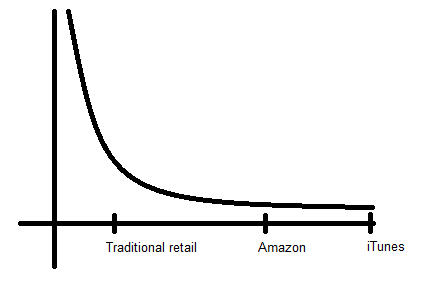
\includegraphics[width=250px]{img/longtail}%
	\end{center}
	\caption{The long-tail: Items ordered by popularity are layed out against their popularity rating. Most of the items reside in the long tail of the graph. Companies such as Amazon can offer a vastly greater subset of the total item space.}%
	\label{figure:longtail}%
\end{figure}

The success of recommender systems to achieve this objective has been the subject of some research, e.g. \cite{levy:2010} and \cite{celma:2008:phd}. Different classes of recommender algorithms favour different properties\cite{burke:2002, shani:2011:9780387858197}. This is elaborated further in subsection \ref{chapter:literature_study:section:computer:subsection:challenges}. For now its enough to see that the quality of recommendations is not uniquely defined. For example, in order to increase coverage of the item space, achieving high serendipity and novelty may be desired more than high recommendation accuracy, depending on the application context\cite{shani:2011:9780387858197, tripathi:2011, celma:2008:phd}.

Typical applications of recommender systems are product recommenders for online retailers, movie and music recommenders such as \emph{Netflix}\footnote{\url{http://www.netflix.com/}} and \emph{Last.fm}\footnote{\url{http://www.last.fm/}}, and news article recommenders in online news services\cite{levy:2010, rajaraman:2012, celma:2008:phd}.

Recommender system have opened up new possibilities in the landscape of online retail, and as a result, spurred the interest of businesses in this field. A remarkable initiative was the Netflix challenge\index{Netflix challenge}. In 2006, Netflix Inc. offered a prize to beat the performance of their recommendation algorithm by 10 percent. It gave a significant boost to the research on recommendation algorithms, and yielded a winning algorithm in September 2009\cite{bell:2007, rajaraman:2012}.


\subsection{Properties of recommendation algorithms}\label{chapter:literature_study:section:computer:subsection:properties}

in \cite{herlocker:2004:ECF:963770.963772} and \cite{shani:2011:9780387858197}, Herlocker et al. and Shani et al.  respectively, compare the performance of recommender systems. They list a number of metrics for recommendation algorithms. The resulting set of properties consist out of the following characteristics:

\begin{itemize}
	\item \textbf{Accuracy}: The accuracy of item recommendations. There are three broad classes of prediction accuracy measures:
	\begin{itemize}
		\item the prediction of the rating given by a user;
		\item the prediction whether or not a user will actually use the item (for example adding to a queue) opposed to predicting the rating itself;
		\item the prediction of a ranking among items rather than an explicit rating of each item independently.
	\end{itemize}
	\item \textbf{User preference}: The opinion of certain users may be more valuable than the opinion of others.
	\item \textbf{Coverage}: The proportion of items that the recommender system can recommend is referred to as catalog coverage. Another measure in this respect is the percentage of all items that are recommended to users. Finally we can also look at the diversity of the recommended items. Coverage can also mean the proportion of users or user interactions for which the system can recommend items.
The cold start problem relates to coverage as it measures the coverage for a specific type of users, namely new users.
	\item \textbf{Confidence}: Confidence in the recommendation can be defined as the systems trust in its recommendations or predictions. The most common measurement of confidence is the probability that the predicted value is indeed true, or the interval around the predicted value where predefined portion of the true values lie. Confidence bounds can be used to filter recommended items where the confidence in the predicted value is below some threshold.
	\item \textbf{Trust}: Trust refers to the user's trust in the system, as opposed to confidence.
	\item \textbf{Novelty}: Novel recommendations are recommendations for items that the user did not know about.
	\item \textbf{Serendipity}: Serendipity is a measure of how surprising the successful recommendations are. One can think of serendipity as the amount of relevant information that is new to the user in a recommendation, or alternatively as deviation from the 'natural' prediction.
	\item \textbf{Diversity}: Diversity is generally defined as the opposite of similarity. Note that an increase in diversity may correlate to a decrease in accuracy.
\end{itemize}


\subsection{A classification of recommendation algorithms}\label{chapter:literature_study:section:computer:subsection:algorithms}

Based on classifications presented in \cite{burke:2002} and \cite{celma:2008:phd}, a categorization of different types of recommendation strategies can be identified. We will only discuss the two most prominent ones, namely collaborative filtering (CF)\index{recommendation algorithm!collaborative filtering} and content-based filtering (CB)\index{recommendation algorithm!content-based filtering}\cite{herlocker:2000, rajaraman:2012}, and list some hybrid strategies. In the literature on recommender systems other general approaches that are commonly identified, are utility-based filtering, knowledge-based filtering, demographic filtering, and expert-based filtering\cite{burke:2002, bostandjiev:2012}.


\subsubsection{Collaborative recommendation}\label{chapter:literature_study:section:computer:subsection:algorithms:subsubsection:cf}

\emph{Collaborative recommendation}\index{collaborative recommendation|see{collaboratibe filtering}} aggregates item ratings by users. By establishing overlaps between ratings in the corresponding user profiles, the system generates new item recommendations\cite{burke:2002, herlocker:2000}. A typical user profile in a collaborative system consists of a vector of items and their ratings, that continuously augmented as the user interacts with the system over time\cite{burke:2002}. 

For CF-based recommendation\index{CF|see{collaborative filtering}}, there are two classes of entities: users $U$ and items $I$. The data itself can then be represented by a utility matrix\index{utility matrix} $A$. The entries $a_{i,j}$ of the utility matrix represent what is known about the degree of preference of user $u_{i}$ and item $i_{j}$\cite{rajaraman:2012}. As can be seen in figure \ref{figure:utilitymatrix}, the utility matrix will have many blanks as well. The goal of the recommendation algorithm is then to fill in the blanks\cite{rajaraman:2012}.

\begin{figure}%
\begin{center}
	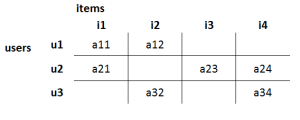
\includegraphics[width=250px]{img/utility_matrix}%
\end{center}
	\caption{The utility matrix $A$.}%
	\label{figure:utilitymatrix}%
\end{figure}

% Similarity / distance functions ...
In order to calculate the blanks, there is a variety of similarity functions that has been developed over the years. Often some sort of distance function is used to compute distance between profile vectors. If the distance is small, profiles will most likely have a high similarity\cite{rajaraman:2012}. The discussion of the mathematics behind each of the algorithms is beyond the scope of this thesis.

% clustering, pearson correlation, ...


\subsubsection{Content-based recommendation}\label{chapter:literature_study:section:computer:subsection:algorithms:subsubsection:cbf}

\emph{Content-based recommendation}\index{content-based recommendation|see{content-based filtering}} learns a profile of the user's interests based on the features present in objects the user has rated. New recommendations can then be generated based on a similarity function on these features\cite{burke:2002, pazzani:2007:CRS:1768197.1768209}.

% Feature vectors ...
When applying content-based filtering, the choice of similarity or classification function will have a significant impact on the quality of the recommendations. More importantly though, is the choice of features. To ensure good performance, these features should also be extracted easily from large quantities of data.

% examples of how feature vectors can be constructed

Depending on the type of item that is being recommended, different approaches can be applied to extract features and construct \emph{feature vectors}\index{feature vector}. Textual information is often extracted using some kind of stemming system\cite{rajaraman:2012}. \emph{Stemming}\index{stemming} is a technique to use root forms that capture a common meaning of certain words, rather than words themselves. For example 'compute', 'computation', 'computer', and 'computes' all have a reference to an underlying concept. Words are given a quantification of relevance to this root form, the so-called TF.IDF (term frequency times inverse document frequency) score\index{TF.IDF}\index{term frequency times inverse document frequency|see{TD.IDF}}. This score is computed in terms of the frequency of the word in a document, number of documents in which it occurs, and the total number of documents. The resulting structure consists out of tuples of root forms and quantification values\cite{pazzani:2007:CRS:1768197.1768209, rajaraman:2012}. The words with the highest scores are the words that characterize the document\cite{rajaraman:2012}. A downside of stemming is that the process may cause the loss of contextual information for each word\cite{pazzani:2007:CRS:1768197.1768209}.

In \cite{bostandjiev:2012} and \cite{melville:2002:CCF:777092.777124} web crawlers are used to gather and extract features from online documents. In \cite{melville:2002:CCF:777092.777124} the web crawler collects properties such as movie title, director, cast, genre, plot summary, plot keywords user comments, reviews and so on, of each movie in the data set. Each property or feature is a 'bag of words'\index{bag of words} that is used in a naive Bayesian text classifier\index{Bayesian classifier}. This way each item can be categorized and the profile can be 'learned'\cite{melville:2002:CCF:777092.777124}.

Tags are very useful as well. Although they can be generated from text, for complex objects such as images and music, tag generation relies on user input\cite{rajaraman:2012}. Nonetheless, emerging technologies such as the 'search by image' option introduced by \emph{Google}\footnote{\url{http://www.google.be/imghp?hl=nl&tab=Ti}}, allow to retrieve web sites, documents and key words related to the given image\cite{google:2011:afbeeldingen}.

Mathematical models of music and images also allow for feature extraction. For example, in a study by Johnson et al. \cite{johnson:2008}, \emph{wavelets}\index{wavelet} were used to construct feature vectors from high resolution paintings. These were in turn used to classify paintings based on several clasification algorithms. A training set of Van Gogh paintings was used with the objective to classify other paitings as either genuine Van Goghs or forgeries. The algorithms were able to actually classify paintings with a high accuracy\cite{johnson:2008}.

Similarly algorithms have been developed to classify music based on content features. There are various types of acoustic features that can be extracted. In \cite{Li:2006:TIM:2219090.2219562} a distinction is made between rhythmic content features, pitch content features and timbral content features.

The research performed by Tzanetakis et al. in \cite{tzanetakis:2001} and \cite{tzanetakis:2002} is based on a the MARSYAS system. This system is an application that uses various techniques, such as Mel-Frequency Cepstral Coefficients (MFCC) and Short-term Fourier Transform Features (FFT) to retrieve acoustic features from audio signals \cite{Tzanetakis:1999:MFA:972850.972857}. In addition to these features, also wavelet-based feature extraction is used to retrieve rhythmic features from audio content \cite{tzanetakis:2001, tzanetakis:2002}. Using this system, music files could be classified into different genres based on rhythmic features\cite{tzanetakis:2001}.

A similar research is conducted by Li et al. in \cite{Li:2006:TIM:2219090.2219562}. In addition to previously mentioned methods, also lyric-based classification is used. Apart from music classification, also music similarity search is performed. In this case, the feature vectors from the classification using MARSYAS features and wavelet-histograms can be used to form a hierarchy in which similar audio signals can be detected \cite{Li:2006:TIM:2219090.2219562}.

% CLassification methods?

%These methods illustrate how mathematical models can be applied for feature extraction, vector generation and classification.


\subsubsection{Hybrid recommendation}\label{chapter:literature_study:section:computer:subsection:algorithms:subsubsection:hf}

\emph{Hybrid filtering}\index{hybrid filtering} combines two or more recommendation algorithms\cite{burke:2002}. In \cite{burke:2002} a number of hybrid recommendation strategies are discussed. Burke et al. list seven different approaches for combining recommendation algorithms:

\begin{itemize}
	\item \textbf{Weighed}: The scores (or votes) of several recommendation techniques are combined together to produce a single recommendation.
	\item \textbf{Switching}: The system switches between recommendation techniques depending on the current situation.
	\item \textbf{Mixed}: Recommendations from several different recommenders are presented at the same time.
	\item \textbf{Feature combination}: Features from different recommendation data sources are thrown together into a single recommendation algorithm.
	\item \textbf{Cascade}: One recommender refines the recommendations given by another.
	\item \textbf{Feature augmentation}: Output from one technique is used as an input feature to another.
	\item \textbf{Meta-level}: The model learned by one recommender is used as input to another.
\end{itemize}

Each of these combinations also has its advantages and disadvantages. Not necessarily all combinations will be successful, and not all of them have been implemented \cite{burke:2002}.



\subsection{Challenges for recommender systems}\label{chapter:literature_study:section:computer:subsection:challenges}

% Cold start / ramp up problem, first rater, new user, new item, gray sheep, profile trust (bad users), sparsity, black box

Each recommendation technique has benefits as well as drawbacks. Some of these apply to all or most types of recommendation strategies, while others are only relevant to certain cases.

Both CF and CB-based recommendation algorithms suffer from the ramp-up\index{ramp-up|see{cold start}} problem in one way or the other. The 'ramp-up' or 'cold start' problem\index{cold start} (although they may refer to slightly different problems depending on the literature) is dual problem that encompasses two distinct, yet related problems as defined in \cite{burke:2002}:

\begin{itemize}
	\item \textbf{New User}\index{cold start!new user}: when a recommender system uses ratings by its users to compute item recommendations, it is hard to find neighbours for a user, who has a limited profile. As user profiles tend to build up over time, new users usually fall in this category.
	\item \textbf{New Item}\index{cold start!new item}: a new item will most likely not have that many ratings associated with it, and as a result will not be easily recommended. This 'new item problem' typically emerges when new items are constantly added to the system; for example when browsing a constant stream of news articles. When new articles are introduced, not many users have had the chance yet to rate these items. In the case of a news feed, an additional problem is that these items are short-lived, meaning that at some point these item profiles will most likely stop receiving any ratings at all.
\end{itemize}

Both of these issues translate themselves into a sparse regions in the utility matrix. It is worth noting that content-based recommendation algorithms suffer less from the \emph{new item} problem, as these tend to rely on features that are inherent to the items themselves, rather than user generated content. This is one of the reasons hybrid approaches can provide a solution to collaborative filtering\cite{burke:2002}. For example, in \cite{melville:2002:CCF:777092.777124}, content-based predictors are used to create pseudo-user ratings to reduce sparsity of the utility matrix, used in a collaborative algorithm.

%Another solution is to use clustering

A problem that is typical of collaborative filtering is the 'gray sheep problem'\index{gray sheep}\cite{burke:2002, herlocker:2000}. The gray sheep problem occurs when a user falls between different clusters of users that may have contradicting item ratings. As a result, it is hard to determine how to classify the user\cite{burke:2002}.

% UV decomposition

Another issue with recommendation systems is that these system often appear as 'black boxes' towards the end user\index{black box}. The complexity of the algorithms used, prevents the user from understanding the recommendation rationale\cite{zhao:2010}. This problem decreases the acceptance by the user of item suggestions. One of the solutions for this problem, proposed by Herlocker et al. in \cite{herlocker:2000}, is to provide an explanation system, i.e., the white box\index{white box}, on top of the recommender system that explains the recommendation process. This can be done through providing a transcript of the system's reasoning or through visualizations\cite{herlocker:2000}.


% more specifics on recommender properties




% ------------------------ The interface --------------------------
% 
% -----------------------------------------------------------------
\section{The interface}\label{chapter:literature_study:section:interaction}

% What will we study?
% Link with previous sections?
In this section we will take a closer look at the visual communication channel.

Shirley et al.\cite{shirley:2009} lists three distinctive limitations:

\begin{itemize}
	\item \textbf{Computational capacity}: time complexity and memory usage of algorithms must allow a responsive user interface, especially in the case of interactive visualization. This is also a requirement to meet the \emph{principle of transparency}\index{principle of transparency} discussed in section \ref{chapter:literature_study:section:user:subsection:interactive:subsubsection:loops3}.
	\item \textbf{Display capacity}: there is a trade-off between the benefits of maximizing the \emph{information density}\index{information density}, i.e., the measure of the amount of encoded information against the amount of unused space, and causing visual overload.
	\item \textbf{Human perceptual and cognitive capacity}: optimizing the cognitive cost is one of the key aspects that make up a successful visualization, as visual and non-visual memory capacity are limited\cite{ware:2004}, as we saw earlier in section \ref{chapter:literature_study:section:user:subsection:interactive}.
\end{itemize}

There has been done extensive research in this domain. Over the last two decades various new information visualization techniques have been developed. These techniques can be classified based on three criteria \cite{keim:2002}:

\begin{itemize}
	\item \textbf{Data}: a classification based on the structure and type of data;
	\item \textbf{Technique}: a classification based on characteristics of visualization techniques;
	\item \textbf{Interaction and distortion}: a classification based on the way in which interaction between user and visualization is enabled.
\end{itemize}


\subsection{Types of data}\label{chapter:literature_study:section:interaction:subsection:datatypes}

% context
% wat can be visualized, data types (recommender data)

Information visualization\index{information visualization}\index{infovis|see{information visualization}} has been focusing on on data sets that lack inherent spatial semantics, thus posing a challenge to map the abstract data onto a two-dimensional screen space\cite{keim:2002}.

There are different types of data and their characteristics will have an influence on the type of visualization. Tables of data consist out of rows, representing items, and columns, representing the data dimensions, or 'attributes'. The number of dimensions is referred to as the dimensionality\index{dimensionality} of the data set\cite{keim:2002}. There are three different kinds of dimensions, namely\cite{shirley:2009}:

\begin{itemize}
	\item \textbf{Quantitative}: numerical data on which arithmetic can be applied;
	\item \textbf{Ordered}: an enumeration that has a definite order;
	\item \textbf{Categorical}: data that has no specific ordering, and is distinguished by name only.
\end{itemize}

Relational data\index{relational data} on the other hand consists out of nodes\index{graph!node} and links or 'edges'\index{graph!edge}\cite{keim:2002, shirley:2009}. Both nodes and edges can have associated attributes.

In \cite{keim:2002} also text and hypertext, and algorithms and software are discussed as examples of other types of data. In the case of text and hypertext, standard visualizations are hard to use, as they cannot be described easily in terms of numbers. As a result, the data is first transformed into description vectors. Next, these vectors can be used in a visualization. Examples of software and algorithm visualization are flow diagrams, presentation using a graph-based structure of source code, and so on\cite{keim:2002}.


\subsection{Visual encoding and visual channels}\label{chapter:literature_study:section:interaction:subsection:encoding}

%Visual encoding principles

\emph{Visual encoding}\index{visual encoding} is defined as the mapping of data set attributes to a visual representation. The choice of visual encoding is one of the central problems in the visualization design\cite{shirley:2009}.

Visual encoding takes place through visual channels. A visual encoding corresponds to a graphical element, or ‘mark’. Examples of visual channels are spatial position, color, size, et cetera. The dimension of the mark may vary: a point is a zero-dimensional mark, a line a one-dimensional one, an area a two-dimensional one and so on.

A visual encoding has the following characteristics, as described in\cite{shirley:2009}:

\begin{itemize}
	\item \textbf{Distinguishability}: the ability of a user to distinguish between visual encodings;
	\item \textbf{Seperability}: Separable visual channels are opposed to integral visual channels, which are focused together on a pre-conscious level. Separable visual channels are safe to use for encoding multiple dimensions;
	\item \textbf{Pop-out}: selecting a channel and make it visually stand out from all the others.
\end{itemize}

%Visual channels

There is a variety of possible visual channels that a visualization designer can turn to in order to create a visual encoding, such as color, spatial position, size, shape, orientation, and so on. The performance of the visual encoding (through a visual channel) depends on the type of data, i.e. quantitative, ordered or categorical \cite{shirley:2009}. Figure \ref{figure:encodings} gives an overview of the performance for each category, adapted from \cite{shirley:2009}. Note that spatial position is the most accurate for each data type.

%Figure 1: Visual encoding performance for each data type
\begin{figure}%
	\begin{center}
		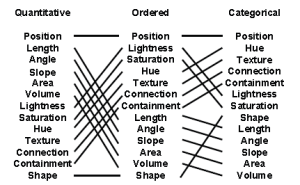
\includegraphics[width=250px]{img/visualencodings}%
	\end{center}
	\caption{Visual encoding performance for each data type, ordered from best to worst.}%
	\label{figure:encodings}%
\end{figure}


%\subsubsection{Colour}\label{chapter:literature_study:section:interaction:subsection:encoding:subsubsection:colour}

In \cite{shirley:2009} colour is considered in terms of three separate channels: \emph{hue}, \emph{saturation} and \emph{brightness}. This allows for different encodings. Just like for most visual channels, the choice of the channel (hue, saturation or brightness) depends heavily on the type of data:

\begin{itemize}
	\item \textbf{Quantitative data}: uses a color map, a range of color values that can be continuous or discrete. It is recommended to use lightness instead of hue, as lightness has an implicit perceptual ordering. Moreover the human eye responds most to strong luminance. Hue on the other hand has a small range (around twelve values that can be reliably distinguished, including background and neutral colors);
	\item \textbf{Ordered data}: lightness and saturation are advised. As mentioned before, these have an implicit perceptual ordering;
	\item \textbf{Categorical data}: hue can be successfully applied for categorical data, keeping in mind its small range.
An important remark is that roughly 10\% of men is red-green color deficient. If a coding uses red and green, it may be wise to apply redundant coding using lightness or saturation in addition to hue \cite{shirley:2009}.
\end{itemize}

Spatial layouts form other visual channels. Although these tend to be the most accurate, spatial layouts in two and three dimensions have several weaknesses \cite{shirley:2009}:

\begin{itemize}
	\item \textbf{Occlusion}: parts of the data set become hidden by others. In the case of the mapping of abstract dimensions onto spatial positions, understanding the details of a three-dimensional visualization may be challenging, even if the user is allowed to change viewpoints;
	\item \textbf{Perspective distortion}: again, in the case of the mapping of abstract dimensions onto spatial positions, distances may convey meaning that may be distorted through perspective.
	\item \textbf{Text in arbitrary orientations}: special care has to be taken with text, as it may become very hard to read depending on the orientation.
\end{itemize}


\subsection{Visualization techniques}\label{chapter:literature_study:section:interaction:subsection:techniques}

% Techniques to overcome limitations of visual channels (see also ware)

Visualization techniques try to deal with the limitations listed in the introduction of this section.



\subsection{Graph-based visualization}\label{chapter:literature_study:section:interaction:subsection:graphs}

% graph-based visualization






% ------------------------ Related work- --------------------------
% 
% -----------------------------------------------------------------
\section{Related work}\label{chapter:survey:section:applications}

In this section we will take a look at visual explanation systems that already exist and that have been evaliated as well. Five different applications are discussed: PeerChooser, Pharos, SFVis, SmallWorlds, and TasteWeights.

Next a comparison is made between these systems, based on a number of objectives for explanation systems listed by Tintarev and Masthoff in \cite{tintarev:2007:SER:1547550.1547664}.


%%%%%%%%%%%%%%%%%%%%%%%%%%%%%%%%%%%%%%%%%%%%%%%%%%%%%%%%%%%%%
%% APPLICATIONS
\subsection{PeerChooser}\label{chapter:survey:section:applications:subsection:peerchooser}

\emph{PeerChooser}\index{PeerChooser} is a "collaborative movie recommender system with an interactive graphical explanation interface"\cite{odonovan:2008}. It aims to address the black box problem, described in section \ref{chapter:literature_study:section:computer:subsection:challenges}\cite{odonovan:2008}.

The application shows a peer graph of the user's neighbourhood. The visualization uses a force-directed graph layout where the on-screen distance between nodes corresponds an approximation of the node similarity. The active user is able to manipulate this neighbourhood by repositioning nodes of the graph. To deal with the high dimensionality of the data, extra cluster nodes are added to the vsiualization. These cluster peer nodes by genre\cite{odonovan:2008}.

By moving a cluster node closer towards the active user's node, all user nodes associated with this cluster will be drawn closer towards the active user node. As a result, these profiles will be temorary considered more similar than before. Similarly individual users can be moved closer towards or further away from the active user node\cite{odonovan:2008}.

Figure \ref{figure:peerchooser} shows the graph-based interface of the PeerChooser application.

\begin{figure}%
	\begin{center}
		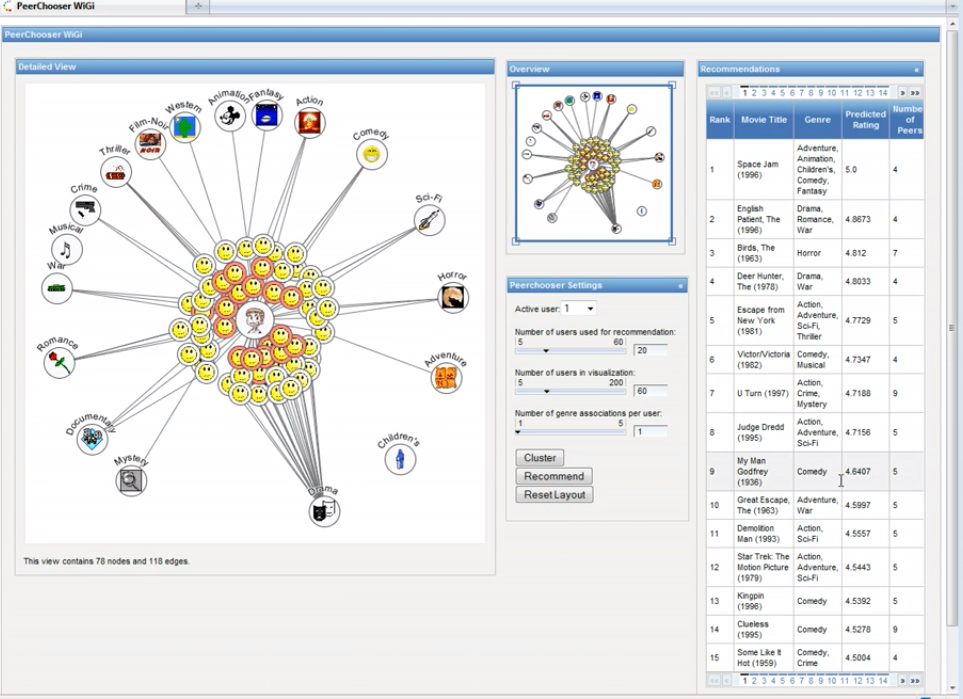
\includegraphics[width=300px]{img/peerchooser}%
	\end{center}
	\caption{The PeerChooser interface.}%
	\label{figure:peerchooser}%
\end{figure}



\subsection{Pharos}\label{chapter:survey:section:applications:subsection:pharos}

Content-centric social websites, such as blogs and discussion forums, contain vast amounts of fast growing information. Recommendation systems have been developed to help users find the information they are looking for. The \emph{Pharos}\index{Pharos} application tries to address two distinctive problems that present themselves in this context: the cold start problem and the black box problem\cite{zhao:2010}, as described earlier in section \ref{chapter:literature_study:section:computer:subsection:challenges}.

As they hope to overcome previously defined problems, Zhao et al. \cite{zhao:2010} collect and visualize content-related social behaviour. The resulting data set is tranformed into a social map. The social map provides a context for new users, addressing the cold start problem. Secondly, the user can explore the social map to increase understanding and user interaction, in an effort to overcome the black box problem.

The generation of the social map takes place through the following three step process:

\begin{itemize}
	\item \textbf{Community extraction}: a map depicting 'which users are talking about what'. Starting from either relationships, people or content communities can be derived;
	\item \textbf{Community/item/people ranking}: the next step is to rank these communities. The 'hotness' can be measured on content, people authorities and so on;
	\item \textbf{Community labeling}: describing what each community is about.
\end{itemize}

An example of what the resulting visualization looks like, is depicted in figure \ref{figure:pharos}.

\begin{figure}%
	\begin{center}
		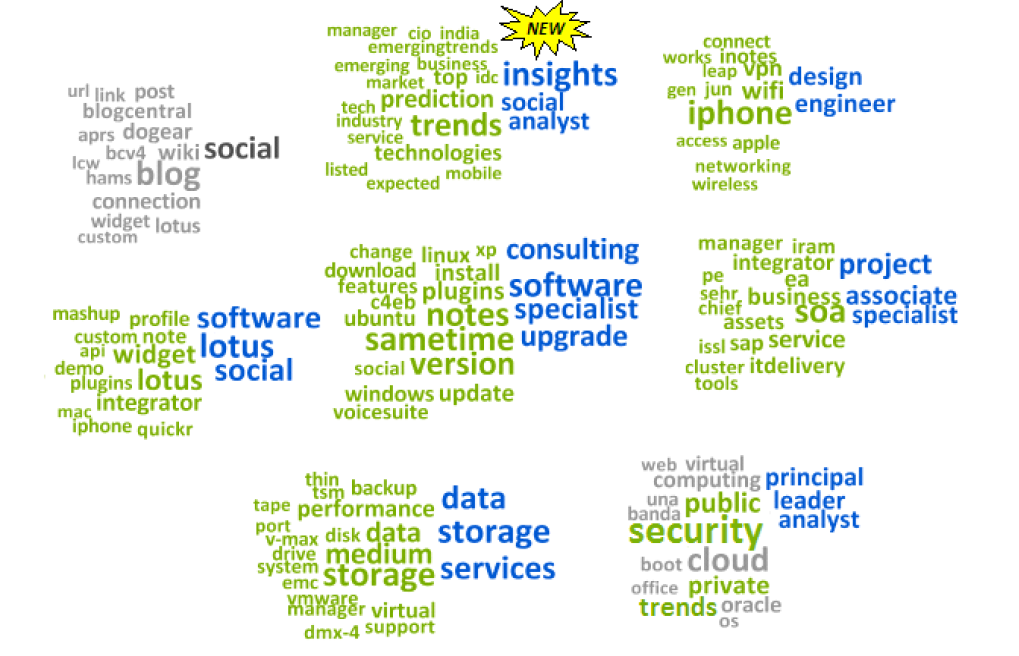
\includegraphics[width=300px]{img/pharos}%
	\end{center}
	\caption{The Pharos social map. Colours indicate activity within a certain group.}%
	\label{figure:pharos}%
\end{figure}




\subsection{SFVis}\label{chapter:survey:section:applications:subsection:sfvis}

SFVis (Social Friends Visualization) is an application that helps users explore and find friends interactively under a context of interest. The system is a hybrid approach of social tags and social networks. The SFVis framework transforms a data model (social tags and social networks) into a visual form. Users can both manipulate the input and visuals on demand.

Social tags can form a network. Within this structure clusters may arise. From this cluster tag network a hierarchy is derived. A compound graph is generated from the tag hierarchy and social networks.

A mapping function assigns actors in a social network to a tag tree. The actor similarity algorithm in SFVis considers both structure similarity in a social network and semantic similarity in a tag network. These scores will allow the recommendation system to compute friend suggestions.

SFVis uses circular visualizations for the different trees and graphs for both views as well as interaction with the user.

\begin{figure}%
	\begin{center}
		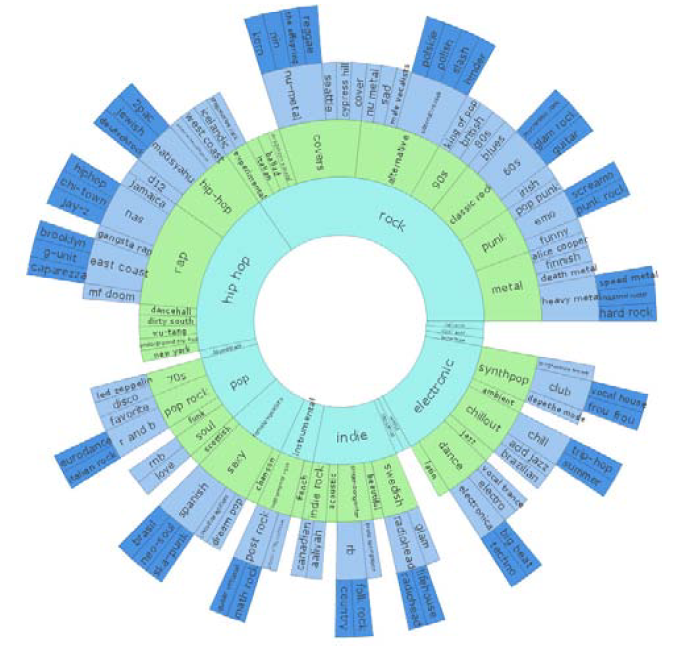
\includegraphics[width=300px]{img/sfviz_tagtree}%
	\end{center}
	\caption{SFViz graphical user interface: tag tree.}%
	\label{figure:sfviz}%
\end{figure}



\subsection{Smallworlds}\label{chapter:survey:section:applications:subsection:smallwords}

In \cite{gretarsson:2010}, Gretarsson et al. used the Facebook API to create an application to generate social recommendations for Facebook users. Unfortunately the Facebook API does not support unauthorized reading of item preference information beyond the immediate friend group. This would not have been a problem unless traditional collaborative filtering strategies tend to produce item suggestions of inferior quality for small items. In this case however the research team relies on the social filtering through the active user's peer group\cite{gretarsson:2010}.

\emph{SmallWorlds}\index{SmallWorlds} is "a visual interactive graph-based interface that allows users to specify, refine and build item-preference profiles"\cite{gretarsson:2010}. The system promotes transparancy in the recommendation process, and gives the user a sense of control over the recommendation process through interactions. This way, Gretarsson et al. try to further overcome the limitations of their recommender system\cite{gretarsson:2010}.

SmallWorlds uses a five-layered design to create suggestions:

\begin{enumerate}
	\item the active user's node;
	\item the active user's profile items;
	\item friends who have items in common with the active user;
	\item items that are not in the active user’s profile, but are liked by friends in layer $3$;
	\item friends who have no items in common with the active user and items in their profiles, but not items in the profiles of friends in layer $3$.
\end{enumerate}

The user can move nodes in each layer further or closer towards the active user's node to adjust the weights of each node. This is used in combination with similarity functions to calculate the suggestions. Figure \ref{figure:smallworlds} shows a screenshot of the application.

\begin{figure}%
	\begin{center}
		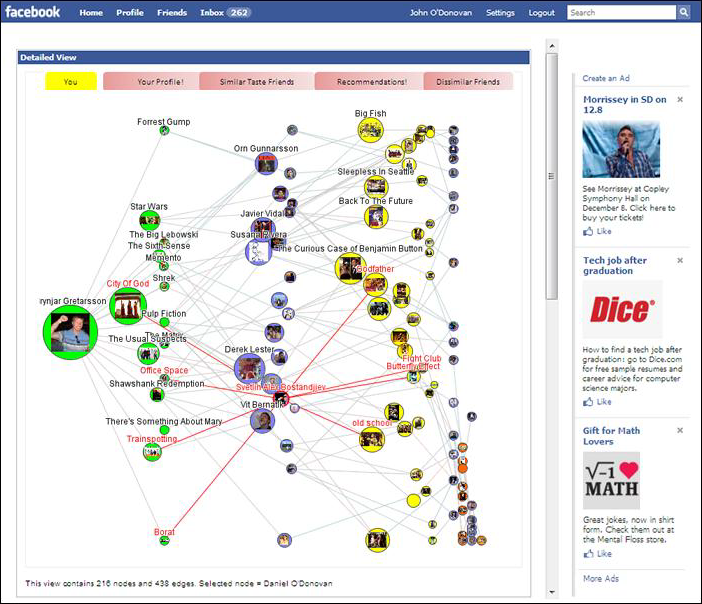
\includegraphics[width=300px]{img/smallworlds}%
	\end{center}
	\caption{The SmallWords interface.}%
	\label{figure:smallworlds}%
\end{figure}


\subsection{TasteWeights}\label{chapter:survey:section:applications:subsection:tasteweights}

TasteWeights is a hybrid recommender with an interactive graphical user interface\cite{bostandjiev:2012}. The application allows the user to express his/her preferences changing the weights of incoming data sources.

One of the challenges Bostandjiev et al. try to address is that "social web APIs and other data sources are constantly evolving, and traditional recommender system techniques such as automated collaborative filtering need to adapt to the changing environment of the social web"\cite{bostandjiev:2012} (cf. Smallworlds). They introduce two enhancements for the traditional techniques. Multiple web sources, namely from \emph{Facebook}\footnote{\url{https://www.facebook.com/}}, \emph{Twitter}\footnote{\url{https://twitter.com/}} and \emph{Wikipedia}\footnote{\url{http://www.wikipedia.org/}} are combined when computing the recommendation. This combination provides a hybrid of different recommendation strategies, namely: collaborative filtering, expert-based and content-based respectively. The second enhancement is a new user interface that provides transparency into the recommendation process.

There are three levels to be distinguished that are represented visually as well:

\begin{itemize}
	\item \textbf{Profile layer}: liked items on \emph{Facebook};
	\item \textbf{Context layer}: items coming from different sources, namely \emph{Twitter}, \emph{Facebook}, and \emph{Wikipedia};
	\item \textbf{Recommendation layer} containing the actual recommendations.
\end{itemize}

Figure \ref{figure:tasteweights} shows the corresponding visual representation of each of these levels. Edges connect relevant parts between each of these levels on the visualization, in an attempt to explain the provenance of item recommendations. The user can influence the outcome displayed in the recommendation layer by attributing weights to the nodes in the profile layer and context layer\cite{bostandjiev:2012}.

\begin{figure}%
	\begin{center}
		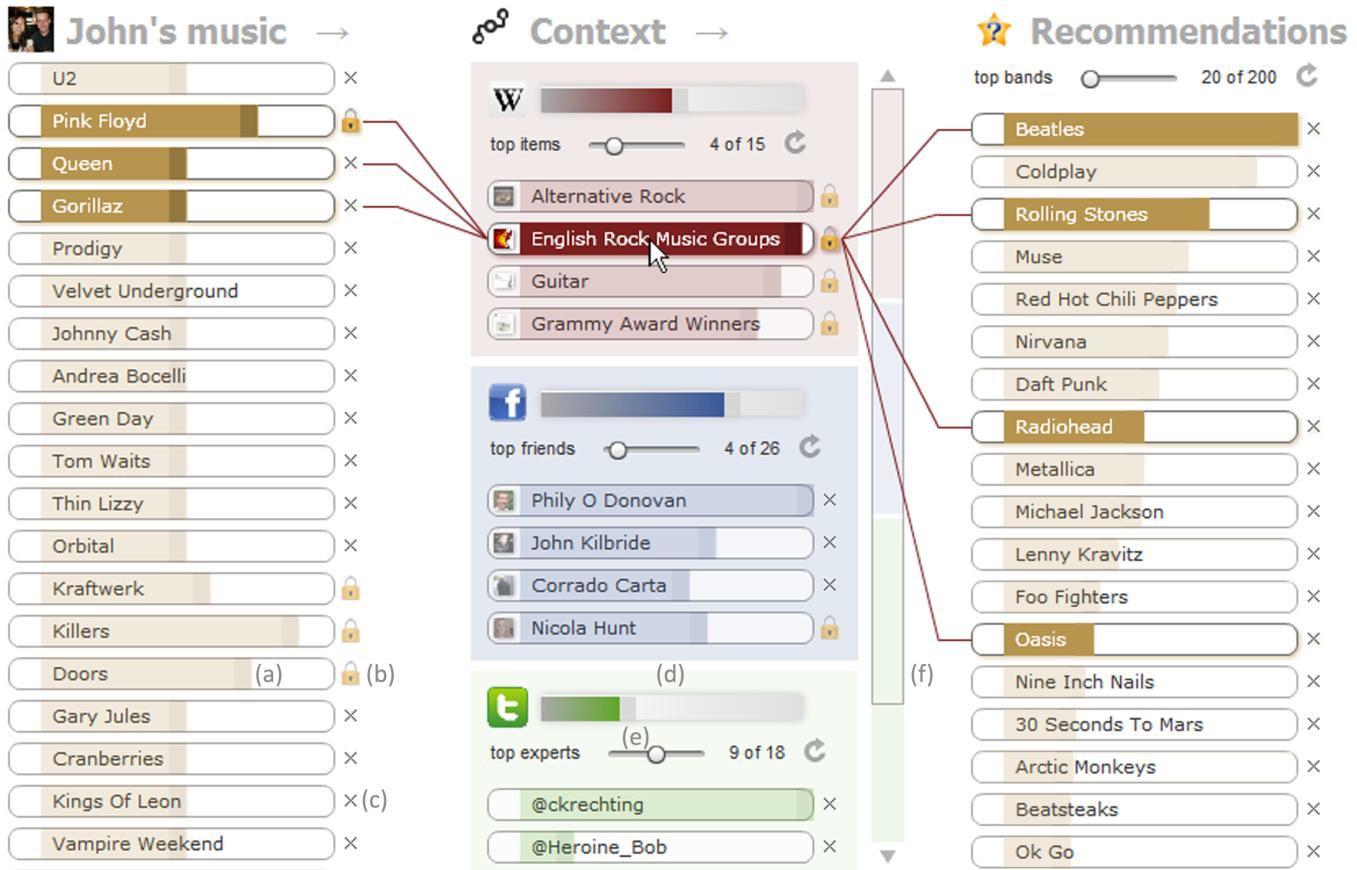
\includegraphics[width=300px]{img/tasteweights}%
	\end{center}
	\caption{The TasteWeights interface.}%
	\label{figure:tasteweights}%
\end{figure}

% research questions: accuracy, user experience, benefit of explanations, hybrid better than CF?







%%%%%%%%%%%%%%%%%%%%%%%%%%%%%%%%%%%%%%%%%%%%%%%%%%%%%%%%%%%%%
%% COMPARATIVE STUDY
\subsection{Comparative study of visual explanation systems for item recommendation}

 The following listing is adapted from \cite{tintarev:2007:SER:1547550.1547664}:

\begin{itemize}
	\item \textbf{Transparency}: explain how the system works;
	\item \textbf{Scrutability}: allow users to tell;
	\item \textbf{Trust}: increase users' confidence in the system;
	\item \textbf{Effectiveness}: help users make good decisions;
	\item \textbf{Persuasiveness}: convince users to try or buy;
	\item \textbf{Efficiency}: help users make decisions faster;
	\item \textbf{Satisfaction}: increase the ease of usability or enjoyment.
\end{itemize}

%Table1 : overview recommender system case studies
In table 1 an overview is presented of some the different recommender systems and some of their properties. So far most of the applications discussed here used collaborative filtering and some kind of visualization and allowed the user to interact with the system.


\chapter{Designing a white box model for collaborative filtering}\label{chapter:whitebox}

In this chapter we will describe our approach to design a white box model for collaborative filtering. In order to provide explanations about the recommendation process, we will base our design on the characteristics of collaborative filtering.

The underlying structure of collaborative filtering can be interpreted as a dual graph. This is a graph $G(V,E)$ for which $V = U \cup I$ such that $U \cap I = \emptyset \wedge E \subseteq U \times I$\cite{dekimpe:2007}. In this case the set of nodes U corresponds to the set of users, and the other set of nodes I is set of items. In plain language this means that there only exist edges of that go from an item to a user or from a user to an item. A quantification of the similarity between users can then be identified as the number of edges leading to common items within user profiles. This way we hope to be able to answer most of the questions raised in the previous paragraphs, describing Herlocker's white box model.

One of the challenges of this approach is overcoming the graph drawing problem, as defined earlier in section \ref{chapter:literature_study:section:interaction:subsection:graphs}. In an application where easily millions of items may be involved, scalability becomes a significant constraint on the visualization design\cite{herman:2000}.

%Several strategies have been identified to reduce the number of items, reduce the number of dimensions and reduce visual clutter, as listed in section \ref{chapter:literature_study:section:interaction:subsection:infovis} and \ref{chapter:literature_study:section:interaction:subsection:graph}.

Based on a visualization design by Valdis Krebs, a dimensionality reduction can be performed on the graph, by keeping only one set of nodes and representing the other set of nodes as implicit information in the edges. In \cite{steele:2010} Valdis Krebs kept the items, books purchased from the Amazon web store in this case, and represented the number of users that where linked to these items, i.e., purchased a particular book, by the thickness of the edges.

\chapter{Iterative development}\label{chapter:prototype}

\section{Methodology}\label{chapter:prototype:section:methodology}



\section{Iteration 1: paper prototype}\label{chapter:prototype:section:paper}



\section{Iteration 2: digital prototype}\label{chapter:prototype:section:digital}



\section{Iteration 3: application implementation}\label{chapter:prototype:section:implementation}



\chapter{Implementation: the SoundSuggest application}\label{chapter:implementation}

The application that was built for this thesis is called \emph{SoundSuggest}. It is a chrome extension that uses the D3 JavaScript library and the Last.fm API to inject the explanation system into the recommendations page of Last.fm\footnote{\url{http://www.last.fm/home/recs}}. In this chapter we will discuss the technologies we have used to create the application, the software design of the application and some specifics about the implementation of the application.


\section{Technologies}\label{chapter:implementation:section:technologies}

\subsection{Chrome extensions}\label{chapter:implementation:section:technologies:subsection:chrome}

Chrome Extensions are applications written in \emph{HTML}\index{HTML}, \emph{JavaScript}\index{JavaScript} and \emph{CSS}\index{CSS}\index{Cascading style sheet|see{CSS}}, that enhance to functionality of the Google Chrome web browser\cite{google:2012:extensions}.

There are different types of extensions. Browser actions are applications that can be launched regardless of the web page you are at. They appear as a button with a specified logo in the toolbar of the Chrome browser. By clicking the browser action you can specify to open up a tooltip or a popup\cite{google:2012:browseraction}. Page action extensions are meant to be shown when browsing specific web pages. They appear as an icon in the address bar. Page actions use content scripts to inject code into the web page\cite{google:2012:overview}.

The file \emph{manifest.JSON} is one of the key areas of a chrome extension. It specifies the name and the version of your application as well as other important settings such as the type of the extension, scripts and security policies\cite{google:2012:manifest}.

Many extensions use a two-layered structure in which you have a background page and UI pages or content scripts\cite{google:2012:overview}. In the usual case the views are stateless and background pages are not. When the view needs some state, it requests the state from the background page. When the background page notices a state change, the background page tells the views to update\cite{google:2012:background}. Background pages can either be persistent or not. In the last case we are talking about so called event pages; they are opened and closed as needed\cite{google:2012:overview}.

There are various ways to use UI pages: you can open an HTML page in a popup, another tab or options page. The HTML pages inside an extension have complete access to each other's DOMs, and they can invoke functions on each other\cite{google:2012:overview}.

Content scripts are JavaScript scripts that are used to interact with a webpage opened in a browser tab. An important remark is that you should consider a content script part of the webpage it is injected into, rather than its parent extension. It can modify the DOM of the webpage but not the DOM of its background page. However it can ask its background page for data through listeners in the background page's script\cite{google:2012:overview}.



\subsection{The Last.fm API}\label{chapter:implementation:section:technologies:subsection:lastfm}

The \emph{Last.fm API}\footnote{\url{http://www.last.fm/api}} offers great functionality such as the recommender system, Last.fm scrobbling and accessing and modifying your Last.fm profile information, aside from providing a large amount of data. To use the API, libraries have been developed for several technologies, such as \emph{JavaScript}\index{JavaScript}, \emph{PHP}, \emph{Python} and \emph{Actionscript} among others\cite{lastfm:2012:home}.

To build an application using the Last.fm API, you have to create an API account first at \url{http://www.last.fm/api/account/create}. Once you have been registered, you will receive an API key and an API secret.

For testing purposes it will also be handy to have a Last.fm account of your own. So if you haven't got one already sign up at their website. You might also want to one or more of their \emph{Scrobbler}\index{Scrobbler} applications. This will collect data from your music players to generate profile information that will be used to generate recommendations\cite{lastfm:2013:scrobbling}.

There are already several interesting applications that make use of the Last.fm API. Even more interesting perhaps is that some developers distribute free JavaScript libraries that act like a facade on the Last.fm API. The JavaScript library we will be using here, can be found on \emph{GitHub}\footnote{\url{https://github.com/fxb/javascript-last.fm-api}} and is written by \emph{Felix Bruns}.


\subsection{D3.js JavaScript Library}\label{chapter:implementation:section:technologies:subsection:d3js}

Visualizations for web applications can be built using \emph{scalable vector graphics}\index{scalable vector graphics} \emph{(SVG)\index{SVG|see{scalable vector graphics}}}. SVG is an XML-based language to describe two-dimensional graphics\cite{w3c:2011:svg}. It is supported by most of the latest versions of most popular browsers, including \emph{Chrome}, \emph{Firefox}, \emph{Internet Explorer 9}, \emph{Opera} and \emph{Safari}\cite{microsoft:2012:svg, w3c:2010:svg}.

\emph{D3.js}\index{D3.js} is a JavaScript library that uses the W3C standards \emph{HTML}, \emph{SVG} and \emph{CSS} to build data-driven documents\index{data-driven documents|see{D3.js}}\cite{bostock:2012:d3js}. There are various tutorials explaining the basics on how to use this library.

In short, to get started the library should be included in your web page. Next, using the D3 selectors, elements can be added and removed easily from the web page. The library also offers a number of built-in algorithms, as well as a series of example visualizations that can be customized as desired.


\subsection{Additional libraries}\label{chapter:implementation:section:technologies:subsection:libs}

In addition to the Last.fm API JavaScript library and D3.js, four other JavaScript libraries were used, namely:

\begin{itemize}
	\item \textbf{jQuery}\footnote{\url{http://jquery.com/}}: "jQuery is a fast, small, and feature-rich JavaScript library. It makes things like HTML document traversal and manipulation, event handling, animation, and Ajax much simpler with an easy-to-use API that works across a multitude of browsers"\cite{jquery:2013}.
	\item \textbf{jQuery UI}\footnote{\url{}}: "jQuery UI is a curated set of user interface interactions, effects, widgets, and themes built on top of the jQuery JavaScript Library"\cite{jqueryui:2013}.
	\item \textbf{Purl.js}\footnote{\url{https://github.com/allmarkedup/jQuery-URL-Parser}}: a library built on the jQuery library to retrieve GET parameters from the web page's URL.
	\item \textbf{Spinner.js}\footnote{\url{http://fgnass.github.io/spin.js/}}: a library that creates a spinner element with given parameters for customization.
\end{itemize}


\section{Software design and application architecture}\label{chapter:implementation:section:design}

% Life lines :
%		ACTOR
%		(UI)
%		content script
%		background script
%		Local storage
%		Last.fm API


\begin{figure}%
	\begin{center}
		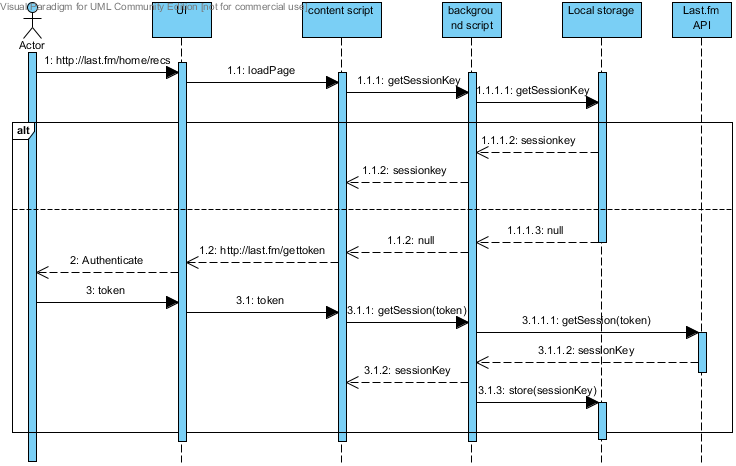
\includegraphics[width=\columnwidth]{img/seq_part1}%
	\end{center}
	\caption{Sequence diagram: opening the Last.fm recommendations page part 1: retrieving a session key.}%
	\label{fig:sequence:part1}%
\end{figure}

\begin{figure}%
	\begin{center}
		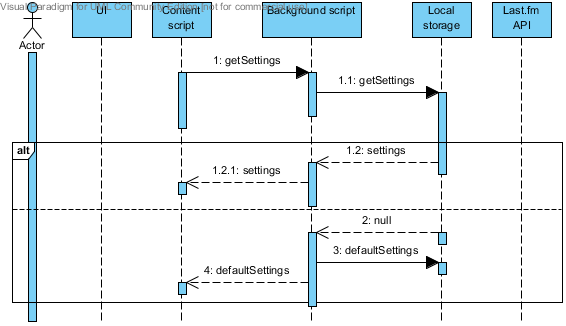
\includegraphics[width=\columnwidth]{img/seq_part2}%
	\end{center}
	\caption{Sequence diagram: opening the Last.fm recommendations page part 2: retrieving stored settings.}%
	\label{fig:sequence:part2}%
\end{figure}

\begin{figure}%
	\begin{center}
		\includegraphics[width=\columnwidth]{img/seq_settings}%
	\end{center}
	\caption{Sequence diagram: changing settings.}%
	\label{fig:sequence:settings}%
\end{figure}



\section{Implementation}\label{chapter:implementation:section:implementation}









\chapter{Conclusion and future work}\label{chapter:conclusion}



% CONTENTS :
% Geef een overzicht van het door jou geleverde werk. Zorg dat het duidelijk is wat je eigen inbreng is en wat je elders gevonden hebt.
% Vergelijk de oorspronkelijke doelstelling met wat je bereikt hebt.
% Vermeld de belangrijkste problemen die je had bij het verwezenlijken van die doelstellingen.
% Wees kritisch en geef de voor- en nadelen van jouw oplossing en vergelijk je bekomen resultaat met beschikbare alternatieven.
% Geef aan welke uitbreidingen en verfijningen je nog zou kunnen/willen doen als je er de tijd voor had.
% 	FUTURE WORK
% 		visualization of content-based recommendation:
%			distance functions of feature vectors in a spatial map
%				...
% 		using this thesis as a starting point with visualization, sensemaking, etc. in literature study
%			using the whitebox in another context than music recommendation



% ------------------------- Bibliography --------------------------
% 
% -----------------------------------------------------------------
%% A small distance to the other stuff in the table of contents (toc)
\addtocontents{toc}{\protect\vspace*{\baselineskip}}

%% The Bibliography
%% ==> You need a file 'literature.bib' for this.
%% ==> You need to run BibTeX for this (Project | Properties... | Uses BibTeX)
\addcontentsline{toc}{chapter}{References} %'Bibliography' into toc
%\nocite{*} %Even non-cited BibTeX-Entries will be shown.
%\bibliographystyle{alpha} %Style of Bibliography: plain / apalike / amsalpha / ...
\bibliographystyle{abbrv}
\bibliography{bib/references}


%% The List of Figures
\clearpage
\addcontentsline{toc}{chapter}{List of Figures}
\listoffigures

%% The List of Tables
\clearpage
\addcontentsline{toc}{chapter}{List of Tables}
\listoftables

%% Index
\clearpage
\addcontentsline{toc}{chapter}{Index}
\printindex


\newpage
% ----------------------- Back cover ------------------------------
% Please fill in:
% - Department
% - Department's address
% - Telephone number and fax number
% - e-mail
% -----------------------------------------------------------------
\thispagestyle{empty}
\sffamily
%
\begin{textblock}{191}(113,-11)
{\color{blueline}\rule{160pt}{5.5pt}}
\end{textblock}
%
\begin{textblock}{191}(168,-11)
{\color{blueline}\rule{5.5pt}{59pt}}
\end{textblock}
%
\begin{textblock}{183}(-24,-11)
\textblockcolour{}
\flushright
\fontsize{7}{7.5}\selectfont
\textbf{AFDELING}\\
Straat nr bus 0000\\
3000 LEUVEN, BELGI\"{E}\\
tel. + 32 16 00 00 00\\
fax + 32 16 00 00 00\\
@kuleuven.be\\
www.kuleuven.be\\
\end{textblock}
%
\begin{textblock}{191}(154,-7)
\textblockcolour{}
\includegraphics*[height=16.5truemm]{sedes}
\end{textblock}
%
\begin{textblock}{191}(-20,235)
{\color{bluetitle}\rule{544pt}{55pt}}
\end{textblock}
\end{document}
